\IEEEraisesectionheading{\section{Introduction}\label{sec:introduction}}

%BACKGROUND
A diverse set of technologies (e.g, algorithms, programming languages, platforms, libraries/frameworks, concepts for software engineering)~\cite{chen2016explore, chen2016techland} is available for use by developers and that set continues growing.
By adopting suitable technologies, it will significantly accelerate the software development process and also enhance the software quality.
But when developers are looking for proper technologies for their tasks, they are likely to find several comparable candidates.
For example, they will find \textit{bubble sort} and \textit{quick sort} algorithms for sorting, \textit{nltk} and \textit{opennlp} libraries for NLP, \textit{Eclipse} and \textit{Intellij} for developing Java applications.
%\textcolor{red}{CCY: Will revise the examples after obtaining all results.}

%POTENTIAL methods
Faced with so many candidates, developers are expected to have a good understanding of different technologies in order to make a proper choice for their work.
However, even for experienced developers, it can be difficult to keep pace with the rapid evolution of technologies.
Developers can try each of the candidates in their work for the comparison.
%, or read documentations, tutorials, examples of each candidate technology.
%\textcolor{blue}{??XINGZC: How about official documentation of a technology? They will describe what the technology is good for. There are two papers ``Patterns of knowledge in API reference documentation'' and ``A field study of API learning resources''. The first one shows that quality and environment knowledge is almost never present and explains that this knowledge remains tacit in the mind of API developers. The second one shows that developers need this type of knowledge to perform their work. At least for API comparison, we can say official documentation is not enough}.
But such trial-and-error assessment is time-consuming and labor extensive.
Instead, we find that the perceptions of developers about comparable technologies and the choices they make about which technology to use are very likely to be influenced by how other developers \textit{see} and \textit{evaluate} the technologies.
So developers often turn to the two information sources on the Web~\cite{bao2017extracting} to learn more about comparable technologies.

First, they read experts' articles about technology comparison like \href{https://dzone.com/articles/why-idea-better-eclipse}{\textit{``Intellij vs. Eclipse: Why IDEA is Better''}}.
Second, developers can seek answers on Q\&A websites such as Stack Overflow or Quora (e.g., \href{https://stackoverflow.com/questions/47011991/apache-open-nlp-vs-nltk}{\textit{``Apache OpenNLP vs NLTK''}}).
These expert articles and community answers are indexable by search engines, thus enabling developers to find answers to their technology comparison inquiries.

\begin{figure}
	\centering
	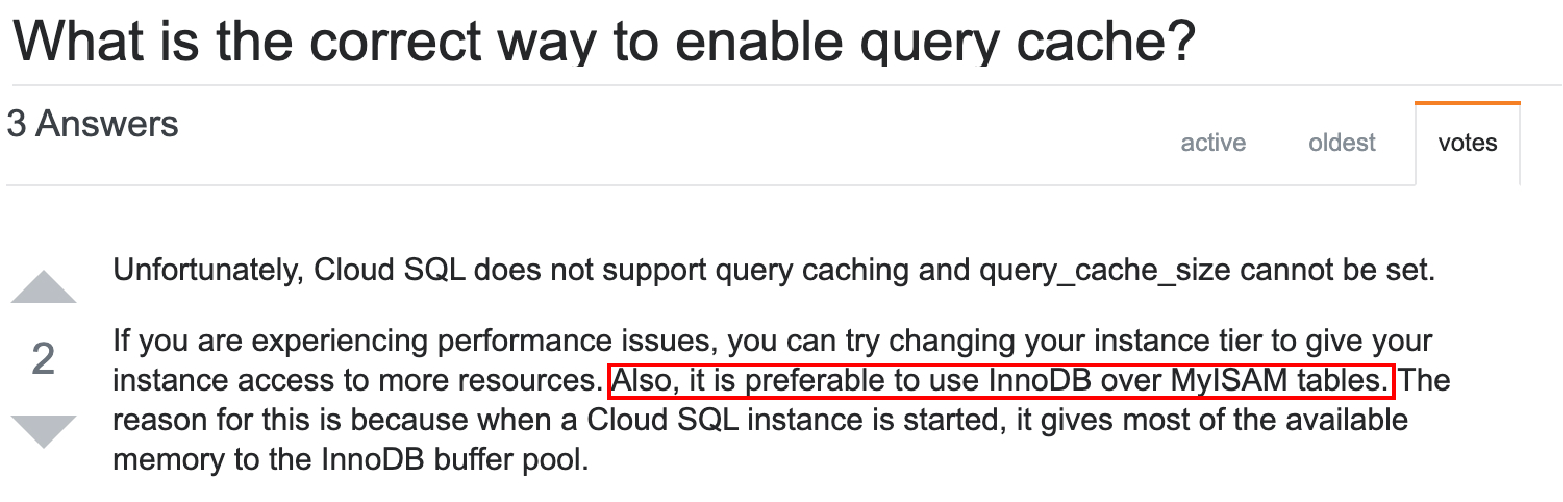
\includegraphics[width=0.47\textwidth]{figures/fig1.pdf}
	
	\vspace{-5mm}
	\caption{A comparative sentence in a question (\#30654296) that is not explicitly for technology comparison.}
	\label{fig:example}
	\vspace{-3mm}
\end{figure}

%LIMITATION of the potential methods
%\textcolor{red}{CCY: I remove two limitations due to their vulnurability, please have a look. In addition, our work cannot also solve the ``diverse opinions'' .}
However, there are two limitations with expert articles and community answers.
%[leftmargin=*]
\begin{itemize}[leftmargin=*]
	%\item \textit{Out of date:} The technology itself is in a constant state of change, while expert articles and community answers, once posted, are rarely updated, leaving the knowledge in them out of date.\textcolor{red}{CCY: Please find some examples to illustrate the first point.}
	
	\item \textit{Fragmented view:} An expert article or community answer usually focuses on a specific aspect of some comparable technologies, and developers have to aggregate the fragmented information into a complete comparison in different aspects.
	For example, to compare \textit{mysql} and \textit{postgresql}, one article~\cite{web:mysql1} contrasts their speed, while another~\cite{web:mysql2} compares their reliability.
	Only after reading both articles, developers can have a relatively comprehensive overview of these two comparable technologies.
	
	%\item \textit{Only intentional comparisons:} Expert articles and community answers cover some technology comparisons that developers intentionally make, but there are much more ``unintended'' knowledge hidden in the Q\&A discussions that do not intentionally discuss or compare technologies. 
	%\item \textit{Personal opinions:} Experts write their own opinions about the similar technologies they use. But their statement of the pros and cons may not be reliable, as the conclusion may be obtained by misusing the technologies or from just personal feelings without hard evidence. 
	%\textcolor{red}{Note that many of these comparative sentences are not present in posts that intentionally discuss or compare two technologies. Instead, hey are widely present when users answer other types of questions. 
	%Fig.\ref{fig:example} shows such as example: the answer ``accidentally'' compares the security of \textit{POST} and \textit{GET}, while the question ``How secure is a HTTP post?'' does not explicit ask for this comparison.
	
	\item \textit{Diverse opinions:} One expert article or community answer is based on the author's knowledge and experience. %??XINGZC: This point could bite back. We fundamentally analyze and summarize community answers. If community answers is questionable because they are opinion-based, then how can our summary be good? Do we have some measurements to tell who are more trustable?}.
	%\textcolor{red}{CCY: We mitigate that problem for three reasons: 1)we only use answers larger than 0 score which means all sentence has been checked by at least one user; 2)we provide multiple comparative sentences for each pair of similar technology, and user can check the crowd opinion rather than one.}
	However, the knowledge and experience of developers vary greatly.
	For example, one developer may prefer \textit{Eclipse} over \textit{Intellij} because \textit{Eclipse} fits his project setting better.
	But that setting may not be extensible to other developers.
	At the same time, some developers may prefer \textit{Intellij} over \textit{Eclipse} for other reasons.
	Such contradictory preferences among different opinions may confuse developers. 
	
\end{itemize}
%Expert articles and community answers have three limitations.

%In this work, we propose a model to aggregate such separated implicit users' opinions as a whole to explicitly compare similar technologies.

%\textcolor{blue}{I formulate the research problem as all the four limitations create difficulties in aggregating information manually. Our approach provides an automated solution to aggregate information.}
The above two limitations create a high barrier for developers to effectively gather useful information about technology differences on the Web in order to tell apart comparable technologies.
Although developers may manually aggregate relevant information by searching and reading many web pages, that would be very opportunistic and time consuming.
To overcome the above limitations, we present the \textit{diffTech} system that automatically distills and aggregates fragmented and trustworthy technology comparison information from the crowd-scale Q\&A discussions in Stack Overflow, and assists technology comparison with an informative summary of different aspects of comparison information.
%Note that the technology differences our system aggregates may be originally scattered in many posts that do not intentionally compare technologies.

Our system is motivated by the fact that a wide range of technologies have been discussed by millions of users in Stack Overflow~\cite{chen2016towards}, and users often express their preferences toward a technology and compare one technology with the others in the discussions.
Apart from posts explicitly about the comparison of some technologies, many comparative sentences \textbf{hide} in posts that are implicitly about technology comparison.
Fig.\ref{fig:example} shows such an example: the answer ``accidentally'' compares \textit{Innodb} and \textit{Myisam}, while the question ``What is the correct way to enable query cache?'' does not explicit ask for this comparison.
Inspired by such phenomenon, we then propose our system to mine and aggregate the comparative sentences in Stack Overflow discussions.

As shown in Fig.~\ref{fig:overview}, we consider Stack Overflow tags as a collection of technology terms and first find comparable technologies by analyzing tag embeddings and categories.
\revise{Our system then mines comparative opinions from Q\&A discussions by analyzing sentence patterns, calculating word mover distance~\cite{kusner2015word} and community detection~\cite{girvan2002community} to cluster comparative sentences into different aspects by which users compare the two technologies for user inspection. 
Finally, we fine-tune the BERT~\cite{devlin2018bert} model to summarize overall sentiment from all the comparative sentences for each comparable technology pairs.}
%\textcolor{red}{I think that we hide out-of-date problems.}
%\textcolor{blue}{Our system analyzes the metadata of the posts from which technology comparison information is extracted, such as post time, post score, post owner's reputation score, to distill likely up-to-date and trustworthy information about technology differences ??XINGZC: from your early comment, I think we analyze post score. How about post owner's reputation? May also be a good indicator of information quality. Furthermore, if we mention out of date as a limitation, we better have some ways to deal with it, for example, by considering the post time, more recent, more up to date. Do not need to do any analysis. Just present some metadata information like post time, user reputation score, post score when showing the comparative sentences is enough.}.
%\textcolor{red}{We then locate the comparative sentences that ...}


As there is no ground truth for technology comparison, we manually validate the performance of each step of our approach. 
The experiment results confirm the accuracy of comparable technology identification (90.7\%), and distilling comparative sentences (89.1\%) from Q\&A discussions.
% recall (\textcolor{red}{??\%})
\revise{By manually building the ground truth, we show that our clustering method (word mover distance and community detection) for comparative sentences significantly outperforms other baselines. 
Regarding the accuracy of overall sentiment summarization, our model also boost \chen{??\%} improvement compared with the baselines.
In addition, we also demonstrate the generality of our approach by successfully extracting comparative opinions of comparable technologies in other domain-specific datasets.}


\begin{comment}
Our first task is to \textcolor{red}{find similar technologies in software engineering domain ??XINGZC: should we reference to our similartech and say this paper extends it to broader technologies?}.
\textcolor{blue}{CCY: ASE is double-blind, we cannot say that is our previous work.}
In Stack Overflow, each question is attached with several tags and each tag is a keyword or a software-specific term which shows what topics this questions resolves.
So we take the tags in Stack Overflow as the representatives of technologies.
We adopt word embedding to tag sentences to obtain tag vector which capture the semantic of tags.
In the vector space, the more closed tag vectors, the more similar are the tags.
\end{comment}

%For example, a user may state that a library is better in speed or easier to learn than the other library in one post, which provides detailed opinions on these technologies.
%As a result, these comparative sentences can be very helpful in summarizing technology comparisons.

%\textcolor{blue}{With comparative sentences that compare two technologies directly ??XINGZC: we should explain that such comparative sentences are not just present in posts that intentionally discuss and compare two technologies. Instead, they are widely present when users answer other types of questions. Is this the case? We may need to collect some data to prove this and also show that those non-intentional comparative sentences cover more pairs of technologies and broader points about these technologies than those intentional comparison posts. Otherwise, people may challenge us ``why not just return the accepted or the most voted answers to those intentional comparison posts?''}, \textcolor{red}{CCY: Good point and I added it below in red.} 


%This paper proposes a method to identify and summarize comparative opinions from Stack Overflow automatically.
%A \textit{comparative opinion} is defined as a comparative sentence which compares the one technology with another, while expressing the user's sentiment on a chosen topic such as memory usage, usability, and performance.

\revise{This paper is an extended version of our earlier study~\cite{huang2018tell}, the extension makes the following additional contributions:
\begin{itemize}
	\item Apart from the existing single-sentence patterns, we also take the context and coreference into the consideration for discovering more comparative sentences about similar technologies.
	%Our model can not only spot the similar technologies, but also their differences.
	\item To give developers an clear overview, we develop a classifier for identifying the sentiment towards each technology, and aggregate the crowd opinions in total.
	\item Based on the extracted comparative opinions, we implement a practical website\footnote{\url{https://difftech.herokuapp.com/}} for developers looking for technology comparison knowledge. The analysis of site visiting logs demonstrate the usefulness of our tool. 
	\item  We not only update previous experiments by including new data and new baselines, but also add more detailed analysis of experiments results. We also demonstrate the generality of our method in other domain-specific datasets.
\end{itemize}
}

\begin{figure}
	\centering
	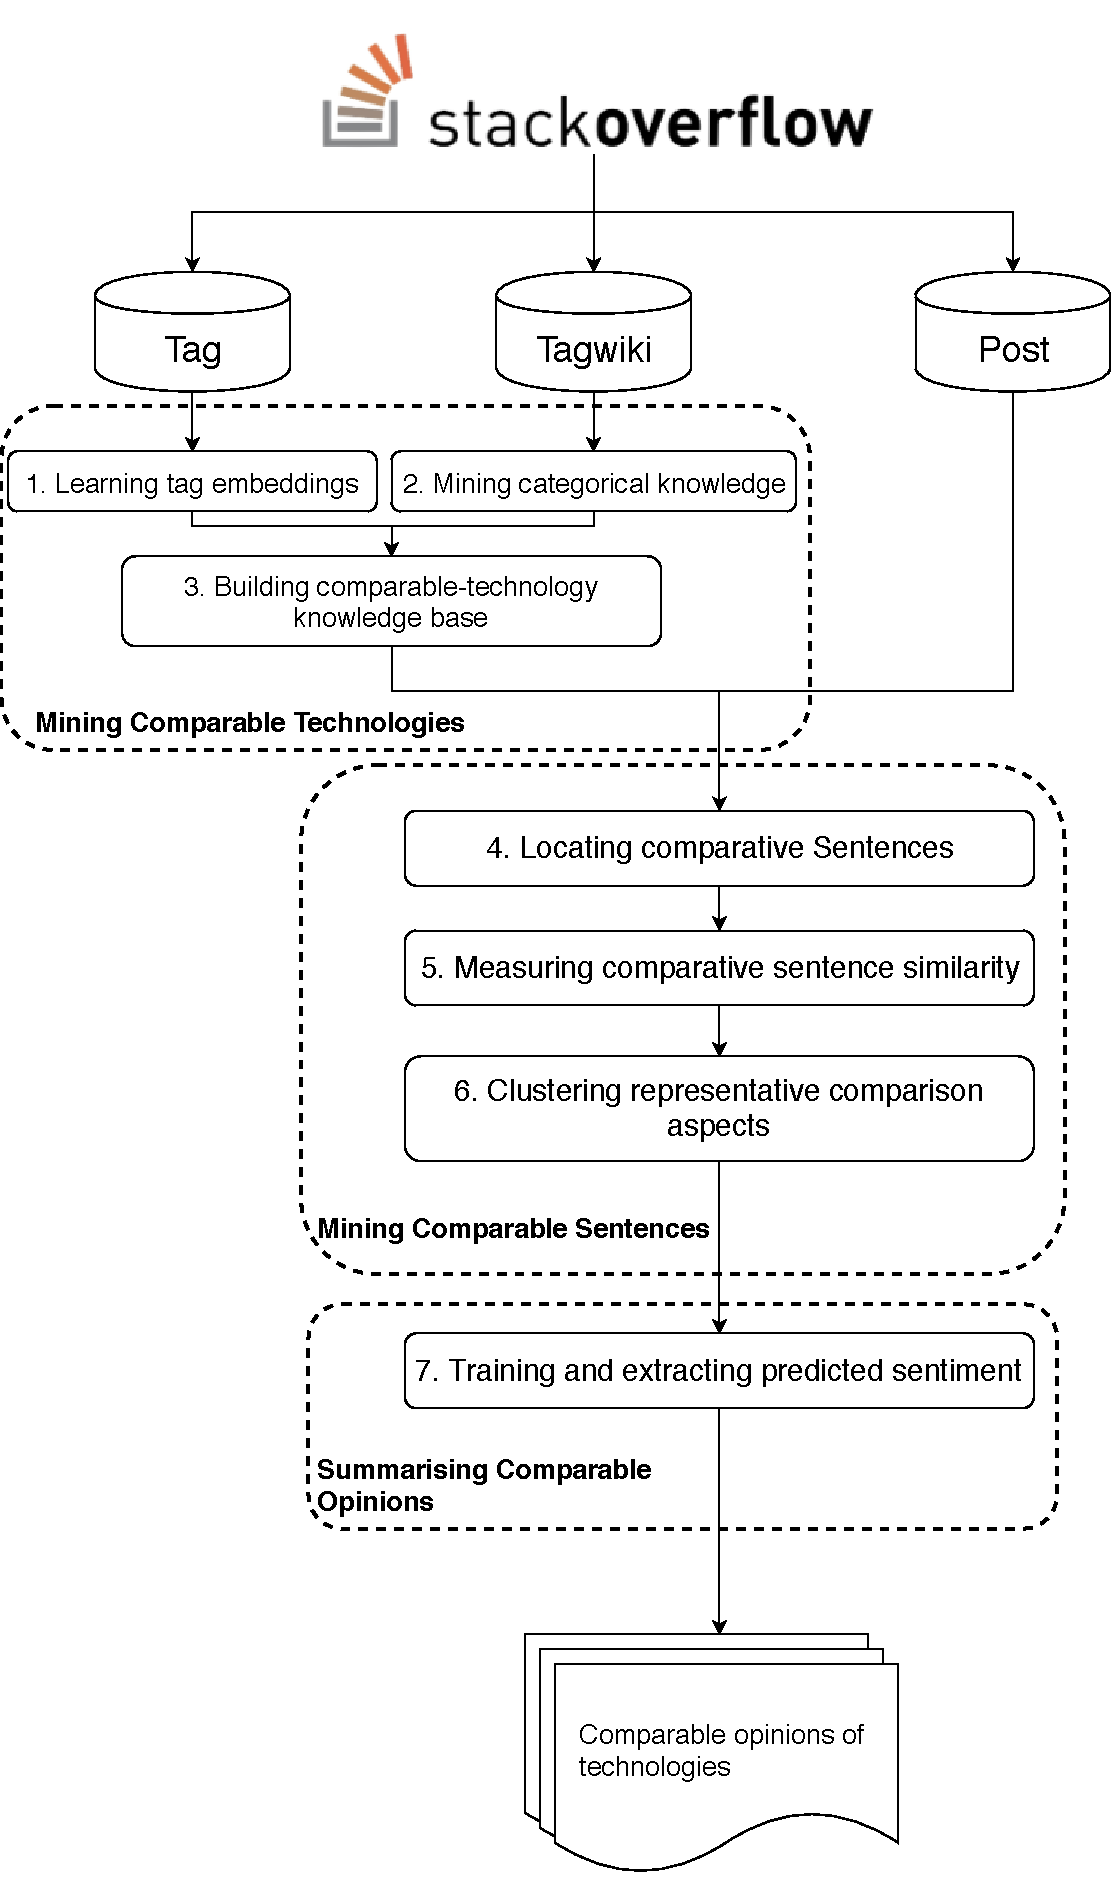
\includegraphics[width=0.48\textwidth]{figures/overview.pdf}
	\vspace{-4mm}
	\caption{The overview of our approach}
	\label{fig:overview}
	\vspace{-3mm}
\end{figure} 